\chapter{L'électrodynamique}
\section{Les équations de Maxwell}
Soit les densités de charges $\rho$ et de courant $\vec{J}$. Ces équations 
s'écrivent \textbf{dans le vide}
\begin{equation}
\begin{split}
\rot \vec E(\vec r,t) &= -\frac{\partial\vec{B}(\vec{r},t)}{\partial t}\\
\rot \vec B(\vec r,t) &= \mu_0\vec{J}(\vec r,t) + \epsilon_0\mu_0\frac{\partial \vec E
(\vec r,t)}{\partial t}\\
\div \vec{B}(\vec r,t) &= 0\\
\div \vec{E}(\vec r,t) &= \frac{\rho(\vec r,t)}{\epsilon_0}
\end{split}
\end{equation}
où $\epsilon_0 = \frac{10^{-9}}{36\pi}\ F/m$ et $\mu_0 = 4\pi 10^{-7}\ H/m$.
Celles-ci sont locales : en un $\vec{r}$ et $t$ donnés. Souvent, à l'endroit où l'on 
souhaite résoudre ces équations il n'y a pas de $\rho$ et $\vec{J}$. Dès lors, à 
l'instant $t$ :
\begin{equation}
\begin{split}
\rot \vec E(\vec r,t) &= -\frac{\partial\vec{B}(\vec{r},t)}{\partial t}\\
\rot \vec B(\vec r,t) &= \epsilon_0\mu_0\frac{\partial \vec E
(\vec r,t)}{\partial t}\\
\div \vec{B}(\vec r,t) &= 0\\
\div \vec{E}(\vec r,t) &= 0
\end{split}
\end{equation}
Ces équations sont bien locales ; les champs satisfont à cette équation, mais il faut bien avoir 
une source quelque part : il y en a forcément (au moins) une, mais elle n'apparaît 
pas localement.\\

\danger Il peut exister $\vec J$ en un point en l'absence de $\rho$ en ce point, car $\rho$ est 
la densité \textbf{totale} de charge en un point : on somme toutes les charges + et - ce qui 
donne un résultat généralement nul. C'est typiquement le cas dans un fil conducteur ou le 
courant circule, mais $\rho = 0$. Cependant, $\vec{J}$ et $\rho$ sont liés par l'équation de 
continuité
\begin{equation}
\div \vec{J}(\vec{r},t) = -\dfrac{\partial\rho(\vec{r},t)}{\partial t}
\end{equation}
Considérons un fil traversé par un courant. Si la quantité sortante est inférieure à la 
quantité entrante, il y a accumulation : c'est ce que nous montre cette équation.\\

Tenir compte du milieu est difficile (courant, charges de polarisation, \dots). Pour régler 
ça facilement, on procède à un astuce mathématique en remplaçant $\mu_0$ et $\epsilon_0$ par 
$\mu$ et $\epsilon$ possédant les caractéristique du milieu. Il s'agit d'un formalisme plus 
simple, mais la physique se voit être "cachée".

\newpage
\subsection{La statique}
Dans ce cas, on obtient deux équations d'électrostatique et deux équations de magnétisme 
\begin{equation}
\begin{array}{ll}
\rot \vec{E}(\vec{r}) = 0,\qquad & \div \vec{E}(\vec{r}) = \dfrac{\rho(\vec{r})}{\epsilon_0}\\
\rot \vec{B}(\vec{r}) = \mu_0\vec{J}(\vec{r}),\qquad & \div \vec{B}(\vec{r}) = 0
\end{array}
\end{equation}
Pour résoudre ces équations, il existe deux méthodes 
\begin{enumerate}
\item Résolution directe
\item Méthode des potentiels
\end{enumerate}
La première méthode n'étant efficace que pour des géométries simples, intéressons-nous à la 
seconde méthode. La petite difficulté est qu'il faut considérer en plus des équations le 
potentiel scalaire $V$ et vecteur $\vec{A}$. Il suffit de voir ceci comme une méthode de 
résolution des ED sans donner plus d'importance à ces potentiels. Pour résoudre les équations 
il faut premièrement calculer les potentiels 
\begin{equation}
V(\vec{r}) = \frac{1}{4\pi\epsilon_0}\int_\mathcal{D}\frac{\rho(\vec{r}')}{|\vec{r}-\vec{r}'|}dV',\qquad
\vec{A}(\vec{r}) = \frac{\mu_0}{4\pi}\int_\mathcal{D}\frac{\vec{J}(\vec{r}')}{|\vec{r}-\vec{r}'|}dV'
\end{equation}
Et en déduire les champs
\begin{equation}
\vec{E}(\vec{r}) = -\grad V(\vec{r}),\qquad \vec{B}(\vec{r}) = \rot \vec{A}(\vec{r})
\end{equation}
Physiquement, c'est plus facilement interprétable que les équations de Maxwell car on peut 
clairement voir le lien de cause à effet. En effet, si le circuit possède une densité de 
charge $\rho$ et que l'on veut le potentiel scalaire au point $r$, on peut facilement deviner 
que celui-ci sera $\propto \rho$ et diminuera avec la distance. Pour avoir le potentiel en 
tout point, il suffira d'intégrer.

\subsection{L'électrodynamique}
Les équations ne peuvent plus être découplées : "\textit{bon chance}" pour la résolution 
analytique. La méthode des potentiels reste d'application dans un cas général si on déduit 
les champ à partir de :
\begin{equation}
\vec{E}(\vec{r},t) = -\grad V(\vec{r},t)-\dfrac{\partial\vec{A}(\vec{r},t)}{\partial t},\qquad\qquad
\vec{B}(\vec{r},t) = \rot \vec{A}(\vec{r},t)
\end{equation}
où le "terme correcteur" traduit le couplage entre $\vec{E}$ et $\vec{B}$. Jusqu'ici nous 
avions considérer une approche quasi-statique en supposant que $V$ à l'instant 
$t$ dépendait de la densité de charge à ce même instant, de même pour $\vec{A}$ négligeant 
ainsi le temps de propagation.\\

La nouveauté, c'est qu'à partir de maintenant on considérera que s'il y a une cause quelque 
part, l'effet ne peut se faire ressentir qu'ultérieurement. Ainsi $V$ et $\vec{A}$ ne peuvent 
dépendre des sources qu'à un moment un peu ultérieur : le temps de propagation. On peut 
postuler le délai de propagation
\begin{equation}
t_p = \dfrac{|\vec{r}-\vec{r}'|}{c}
\end{equation}
soit la distance divisée par la vitesse de la lumière. Pour tenir compte de ces délais, 
il faut réadapter nos définitions \\
\retenir{\textit{Tout l'électromagnétisme en une box} 
\begin{equation}
V(\vec{r}) = \frac{1}{4\pi\epsilon_0}\int_\mathcal{D}\frac{\rho(\vec{r}',t-\frac{|\vec{r}-\vec{r}''|}{c})}{|\vec{r}-\vec{r}'|}dV',\qquad
\vec{A}(\vec{r}) = \frac{\mu_0}{4\pi}\int_\mathcal{D}\frac{\vec{J}(\vec{r}',t-\frac{|\vec{r}-\vec{r}''|}{c})}{|\vec{r}-\vec{r}'|}dV'
\end{equation}
On les dénomme les \textbf{potentiels retardés}.}

\newpage
Il est utile de savoir lorsque l'approximation quasi-statique peut être utilisée. Soit 
$\tau$ l'échelle de temps caractéristique de variation des sources et $L$ la dimension 
caractéristique du système étudié. Le retard doit être pris en compte s'il est de l'ordre 
du temps caractéristique : $L/c \thicksim \tau$, ou encore
\begin{equation}
L \thicksim c\tau
\end{equation}
Si la source est sinusoïdale de fréquence $f$, on peut considérer que $\tau$ est 
la période d'oscillation ($\tau = 1/f$) de sorte à écrire la précédente équation
\begin{equation}
L \thicksim \frac{c}{f} = \lambda
\end{equation}
En résumé\\
\retenir{La modélisation quasi-statique n’est plus applicable si les dimensions du 
système sont comparables ou supérieures à la longueur d’onde $$L\thicksim \lambda$$
Pour \SI{1}{\giga\hertz}, la longueur d'onde dans le vide vaut \SI{30}{\centi\meter}. On fera ainsi l'approximation quasi-statique lorsque $L/\lambda \ll 1$.}\ \\ \\

\begin{wrapfigure}[10]{l}{5.2cm}
\vspace{-5mm}
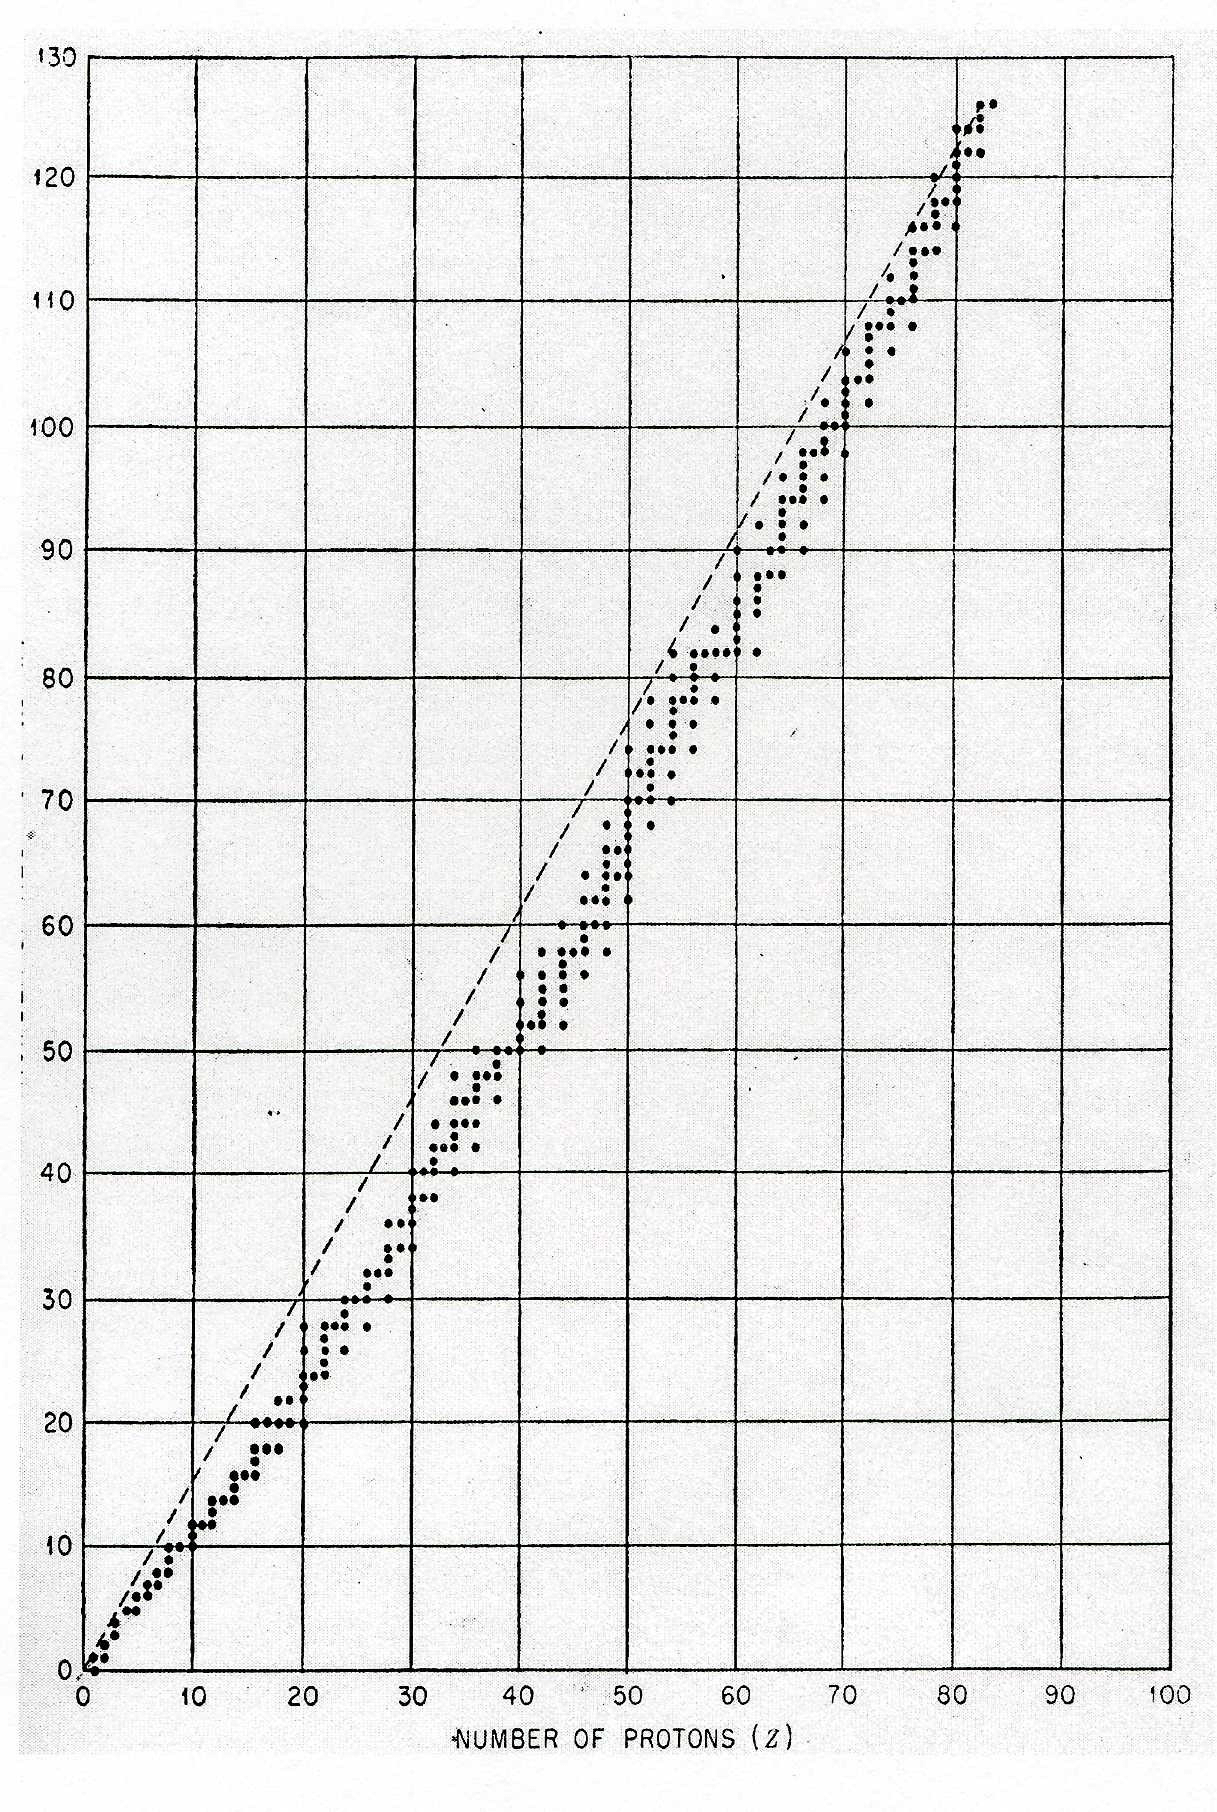
\includegraphics[scale=0.35]{ch1/image1}
\captionof{table}{Régions
du spectre électromagnétique}
\end{wrapfigure}
Nous nous intéresserons à la zone radio/micro-onde ou $\lambda\approx \SI{30}{\centi\meter}$. Pour un 
GSM, la taille de ce-dernier n'est pas négligeable par rapport à ce $\lambda$ de 
même pour le wifi à \SI{5.5}{\giga\hertz} où $\lambda\approx \SI{12}{\centi\meter}$. C'est aussi vrai dans l'infrarouge, 
mais il existe un formalisme plus simple à hautes fréquences.\\

"\textit{En fait, passer de la quasi-statique à l'électrodynamique revient à déplacer 
la modélisation physique des charges et courants vers les champs.}"


\section{Énergétique}
\subsection{L'énergie électrique}
Il existe dans tout l'espace une densité d'énergie électrique, venant de la "séparation" 
des charges électriques (énergie potentielle pouvant être libérée) :
\begin{equation}
w_e(\vec{r},t) = \frac{1}{2}\epsilon|\vec{E}(\vec{r},t)|^2
\end{equation}
On obtient l'énergie électrique du système de charge par intégration.

\subsection{L'énergie magnétique}
Déplacer des charges pour créer un courant exige de fournir un travail stocké sous 
la forme "d'énergie cinétique" : on définit une densité d'énergie magnétique :
\begin{equation}
w_m(\vec{r},t) = \frac{1}{2\mu}|\vec{B}(\vec{r},t)|^2
\end{equation}
























